\section{Durchführung}
\label{sec:Durchführung}

\subsection{Versuchsaufbau}
\label{sec:aufbau}
Der Versuchsaufbau ist in Abbildung \ref{fig:roehre} zu sehen.
Dieser besteht aus einer Röntgenröhre, dessen Strahlung in Richtung einer Halterung emittiert wird.
In dieser Halterung wird ein LiF-Kristall befestigt, welcher in verscheidenen Winkel in Bezug auf die Strahlung ausgerichtet werden kann.
Zudem ist an der Halterung ein Geiger-Müller-Zählrohr angebracht.
Dieses kann ähnlich wie der Krsitall in einem wählbaren Winkel zur Strahlung ausgerichtet werden, die von dem Kristall reflektiert wird.
Die Beschleunigungsspannung an der Röntgneröhre beträgt $U_\text{B} = \SI{35}{\volt}$ und der Emissionsstrom hat eine  Wert von $\SI{1}{\milli\ampere}$.
Es wird eine $1\si{\milli\meter}$ Blende für die Röntgneröhre benutzt.
Auf das Geiger-Müller-Zählrohr wird eine waagerechte Schlitzblende gesetzt.
\begin{figure}
    \centering
    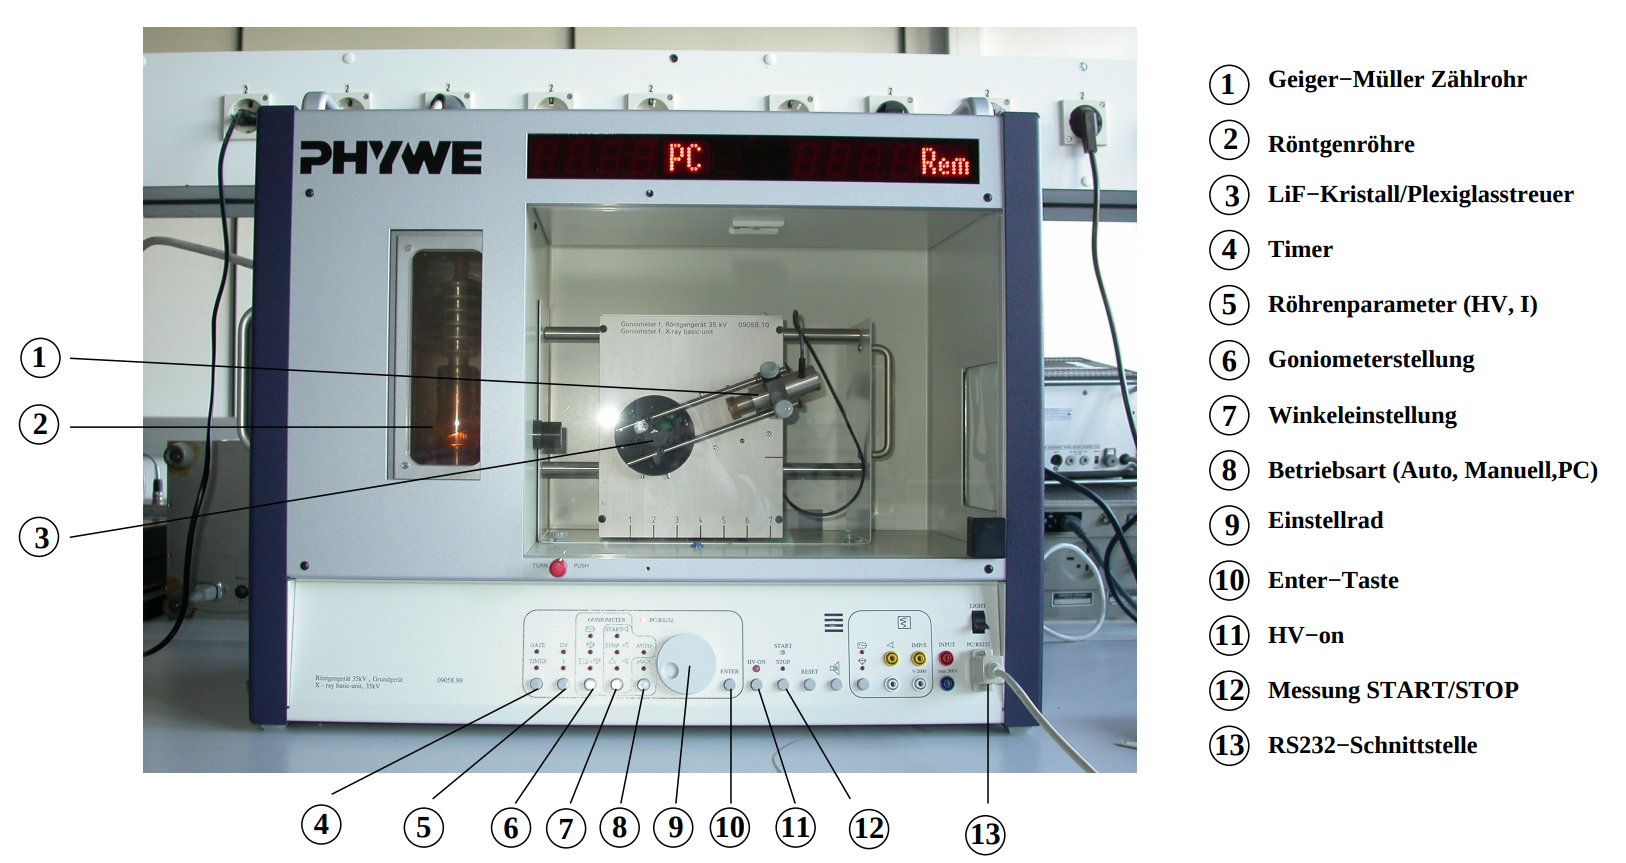
\includegraphics[width=\textwidth]{content/data/Roehre.png}
    \caption{Der Versuchsaufbau entnommen aus der Versuchsanleitung \cite{anleitung}.}
    \label{fig:roehre}
\end{figure}


\subsection{Versuchsdurchführung}
\subsubsection{Bragg-Bedingung}
\label{sec:bragg}
Zunächst wird die Bragg-Bedingung überprüft.
Dafür wird der LiF-Kristall auf einen Winkel von $\theta = 14\si{\degree}$ gestellt.
Nun wird das Geiger-Müller-Zählrohr so eingestellt, dass es in einem Winkel von $\alpha_\text{GM} = 26 \si{\degree}$ steht.
Die Röntgenröhre wird eingeschaltet und die Intensität der Strahlung wird mit einer Integrationszeit von $\Delta t = 5 \si{\second}$ gemessen.
Nach der Messung wird der Winkel $\alpha_\text{GM}$ um $0.1\si{\degree}$ erhöht und die Messung wird erneut durchgeführt.
Der Prozess wird bis zu einem Winkel von $\alpha_\text{GM} = 30\si{\degree}$ wiederholt.

\subsubsection{Emissionsspektrum einer Cu-Röntgneröhre}
\label{sec:emission}
Nun wird an der Apparatur das Programm '2:1 Koppelmodus' ausgewählt und der Winkel des LiF-Kristall wird auf $\theta = 8 \si{\degree}$ gesetzt.
Die Intensität der Röntgenstrahlung wird wieder mit einer Integrationszeit von $\Delta t = 5 \si{\second}$ gemessen.
Nach der Messung wird der Winkel $\theta$ des Krsitalls um $0.1 \si{\degree}$ erhöht.
Die Messung wird wiederholt bis $\theta$ $25\si{\degree}$ erreicht hat.

\subsubsection{Absorptionsspektrum}
\label{sec:abso}
Zuletzt wird das Absorptionsspektrum einiger Stoffe gemessen.
Dafür wird vor das Geiger-Müller-Zählrohr ein Absorber eingesetzt.
Die Absorber bestehen aus Zink, Brom, Gallium, Rubidium, Zirkonium und Strontium.
Die Absorptionsspektren werden in $0.1\si{\degree}$-Schritten, bei einer Integrationszeit von $\Delta t = 20 \si{\second}$ gemessen.
Nach der Messung eines Absorptionsspektrums wird der Absorber durch einen anderen ausgetauscht bis alle Spektren gemessen wurden.
